\documentclass[12pt,a4paper]{article}
\usepackage[a4paper,left=20mm,right=15mm,top=18mm,bottom=20mm]{geometry}
\usepackage{fontspec}
\defaultfontfeatures{Ligatures=TeX}
\setmainfont{PT Sans}
\setsansfont{PT Sans}
\setmonofont{PT Mono}[Scale=0.88]

\usepackage[table]{xcolor}
\definecolor{Brand}{HTML}{1A2AF4}
\definecolor{BrandDark}{HTML}{111EAD}
\definecolor{LetyTechBlue}{HTML}{1A2AF4}
\definecolor{LetyTechPattern}{HTML}{E2E5F0}
\definecolor{Success}{HTML}{237A57}
\definecolor{Light}{HTML}{F3F5FF}
\definecolor{Muted}{HTML}{53617D}

\usepackage{graphicx}
\usepackage{tikz}
\usepackage{array}
\usepackage{tabularx}
\usepackage{longtable}
\usepackage{booktabs}
\usepackage{fancyhdr}
\usepackage{hyperref}

\renewcommand{\figurename}{Рисунок}

\hypersetup{
  colorlinks=true,
  linkcolor=BrandDark,
  urlcolor=Brand,
  pdftitle={Техническое задание: рабочий прототип мобильного сканера},
  pdfauthor={Проектная команда CRM\_14}
}

\pagestyle{fancy}
\fancyhf{}
\fancyhead[L]{\small\color{Brand}\bfseries ЛЭТУ.ТЕХ \textbar\ МИРЭА хакатон 26 \textbar\ Техническое задание CRM-14}
\fancyhead[R]{\small\color{Muted}JavaТСД}
\fancyfoot[C]{\thepage}
\renewcommand{\headrulewidth}{0.3pt}
\setlength{\headheight}{14pt}

\setlength{\parindent}{0pt}
\setlength{\parskip}{5pt}
\setlength{\emergencystretch}{3em}
\sloppy
\renewcommand{\arraystretch}{1.22}
\setcounter{tocdepth}{2}

\newcolumntype{Y}{>{\raggedright\arraybackslash}X}
\newcolumntype{L}[1]{>{\raggedright\arraybackslash}p{#1}}

\newcommand{\status}[1]{\textcolor{Success}{\textbf{#1}}}
\newcommand{\code}[1]{\texttt{#1}}
\newcommand{\placeholder}[1]{\textcolor{Muted}{\textit{[Заполнить: #1]}}}
\newcommand{\screenplaceholder}[1]{%
  \begin{center}
  \fcolorbox{Muted}{Light}{\begin{minipage}[c][52mm][c]{0.82\textwidth}\centering\color{Muted}\textbf{Место для экрана}\par\smallskip\placeholder{#1}\end{minipage}}
  \end{center}%
}
\newcommand{\phonescreen}[3]{%
  \begin{minipage}[t]{0.29\textwidth}
    \centering
    \IfFileExists{#2}{%
      \includegraphics[width=\linewidth,height=62mm,keepaspectratio]{#2}%
    }{%
      \fcolorbox{Muted}{Light}{\begin{minipage}[c][62mm][c]{0.82\linewidth}\centering\color{Muted}\textbf{Скриншот #1}\par\smallskip\placeholder{#3}\end{minipage}}%
    }%
    \par\smallskip\footnotesize\textbf{#1.} #3
  \end{minipage}%
}
\newcommand{\req}[4]{%
  \subsubsection*{#1. #2}
  \addcontentsline{toc}{subsubsection}{#1. #2}
  \textbf{Требование.} #3

  \textbf{Критерий проверки.} #4
}

\newenvironment{infobox}
{\begin{center}\begin{minipage}{0.92\textwidth}\color{BrandDark}\textbf{Примечание}\par\smallskip}
{\end{minipage}\end{center}}


\begin{document}

\begin{titlepage}
  \pagecolor{LetyTechBlue}
  \color{white}
  \thispagestyle{empty}
  \vspace*{16mm}
  {\fontsize{21}{24}\selectfont\bfseries ПРОЕКТНАЯ ДОКУМЕНТАЦИЯ\par}
  \vspace{4mm}
  \vfill
  {\raggedright\fontsize{30}{36}\selectfont\bfseries Рабочий прототип мобильного сканера для сотрудников\par}
  \vspace{7mm}

  \vfill
  \begin{tabular}{@{}ll@{}}
    Дата: & 11 сентября 2026 г. \\
    Команда: & CRM\_14 \\
    Тимлид: & Кармаев Андрей Александрович, ИНБО-30-25 \\
    Java разработчик: & Рахимов Шамиль Рашитович, ЭФБО-02-25 \\
    Дизайнер: & Маркина Майя Витальевна, ЭФБО-02-25 \\
    Дизайнер: & Полухина Елизавета Константиновна, ЭФБО-02-25 \\
    Аналитик: & Кучин Иван Вадимович, ЭПБО-01-25 \\
  \end{tabular}
  \vfill
  \vspace*{10mm}
\end{titlepage}
\nopagecolor
\color{black}

\tableofcontents
\clearpage

\section{Паспорт прототипа}

\begin{tabularx}{\textwidth}{L{48mm}Y}
\toprule
\textbf{Поле} & \textbf{Что написать} \\
\midrule
Название прототипа & Мобильный сканер для складских операций (JavaТСД) \\
Проблема & Существующие устройства используют устаревшее ПО, которое трудно сопровождать и расширять. Требуется приложение на Java с доступными исходниками для удобного редактирования и быстрого добавления функций. \\
Пользователь & Складской сотрудник предприятия Л'Этуаль, выполняющий приёмку и размещение товара. \\
Платформа & Android, minSdk 26. \\
Версия & 0.1. \\
\bottomrule
\end{tabularx}

\subsection{Кратко о продукте}

JavaТСД --- Android-приложение на Java для складского сотрудника Л'Этуаль. Оно помогает принимать и размещать товар с помощью сканирования штрихкодов EAN-13. Операционные данные хранятся на устройстве и загружаются из подготовленных файлов импорта.

\section{Назначение и сценарии работы}

\subsection{Назначение продукта}

Основной продукт --- мобильный сканер для складских операций в Л'Этуаль. Он помогает сотруднику открыть подготовленное задание, быстро считать штрихкод товара, проверить данные и подтвердить результат. Справочник товаров, ячейки и задания загружаются в приложение из подготовленных файлов импорта.

\subsection{Пользователи и доступы}

\begin{tabularx}{\textwidth}{L{45mm}Y}
\toprule
\textbf{Роль} & \textbf{Доступ и действия} \\
\midrule
Складской сотрудник & Открывает локально загруженные задания на приёмку или размещение, сканирует товары, проверяет данные и подтверждает выполнение. Видит сведения, необходимые для выполнения текущей операции. \\
\bottomrule
\end{tabularx}

\subsection{Причина разработки}

Используемые устройства работают с устаревшим ПО, которое сложно сопровождать и расширять. Требуется Java-приложение со сканером, которое легко сопровождать и расширять.

\subsection{Границы прототипа и ограничения}\label{scope:limitations}

Цель прототипа --- показать мобильный сканер штрихкодов и понятный порядок действий сотрудника при складских операциях. Приложение считывает код товара или коробки, показывает относящееся к операции задание, дает сотруднику проверить данные и фиксирует подтвержденный результат. Приоритетом являются скорость и надежность сканирования, простой интерфейс для ТСД и независимость бизнес-сценариев от конкретной реализации сканера.

В состав прототипа \textbf{входят}:

\begin{itemize}
  \item экран сканирования штрихкода с обработкой успешного считывания, ошибки и отказа в доступе к камере;
  \item единый интерфейс модуля сканирования, который в дальнейшем позволит заменить камерный сканер на Zebra DataWedge, SDK ТСД или другую реализацию без изменения логики операций.
  \item проверка отсканированного кода в рамках открытого задания и явное подтверждение результата сотрудником;
  \item импорт подготовленных файлов со справочником товаров, ячейками и заданиями;
  \item хранение каталога, заданий, результатов операций и отчётов о приёмке только на устройстве;
  \item сохранение фотографии подписанной накладной в отчёте о приёмке для последующего просмотра документа;
\end{itemize}

В состав прототипа \textbf{не входят}:

\begin{itemize}
  \item интеграция с 1С, ERP, WMS, API поставщиков, корпоративными сервисами или любыми другими внешними учетными системами;
  \item автоматическая синхронизация справочника товаров, остатков, заданий и результатов операций с сервером;
  \item разработка собственной полноценной системы учета товаров, управления остатками, заказами, поставками или складскими ячейками;
  \item серверная часть бизнес-операций, многопользовательская работа, управление ролями, авторизация и централизованное администрирование;
  \item юридически значимый электронный документооборот, электронная подпись и хранение оригиналов документов;
\end{itemize}


\subsection{Общий цикл работы с JavaТСД}

\begin{enumerate}
  \item Сотрудник выбирает подготовленное задание в приложении.
  \item Открывает задание и видит тип операции, зону или ячейку, товар и требуемое действие.
  \item Сканирует EAN-13 товара, при необходимости указывает фактическое количество или подтверждает ячейку.
  \item Подтверждает выполнение; приложение фиксирует результат и сообщает об ошибках или расхождениях.
  \item Приложение сохраняет и показывает итог операции на устройстве. Передача результатов во внешнюю учётную систему не выполняется.
\end{enumerate}

\section{Техническая часть}

\begin{tabularx}{\textwidth}{L{43mm}Y}
\toprule
\textbf{Компонент} & \textbf{Техническое решение} \\
\midrule
Платформа & Android 8.0+ (\code{minSdk 26}), Java; интерфейс для смартфонов и ТСД. \\
Сканирование & ML Kit Barcode Scanning, bundled-вариант, работа без сети. \\
Архитектура & Экран операции $\longleftrightarrow$ бизнес-операция $\longleftrightarrow$ адаптеры сканера и источника данных. \\
Совместимость & Адаптер ML Kit можно заменить на Zebra DataWedge, SDK ТСД или другую реализацию без изменения бизнес-логики. \\
Данные & Справочник товаров, ячейки и задания импортируются из подготовленных файлов. Операционные данные и результаты хранятся только на устройстве. \\
Документы & Фотография подписанной накладной сохраняется в отчёте о приёмке и доступна при его просмотре. \\
\bottomrule
\end{tabularx}

Сканирование возвращает код или ошибку и не изменяет результат операции до явного подтверждения сотрудником. Ошибки распознавания, неподходящий код и отсутствие доступа к камере отображаются понятным сообщением.

\clearpage
\subsection{Модель данных}

Ниже показана основная связь между сведениями о товаре и ячейками склада: \code{local\_inventory\_cache.cell\_id} ссылается на \code{storage\_cells.id}. Справочники, задания, результаты операций и отчёты о приёмке хранятся в локальной базе данных устройства.

\begin{figure}[htbp]
  \centering
  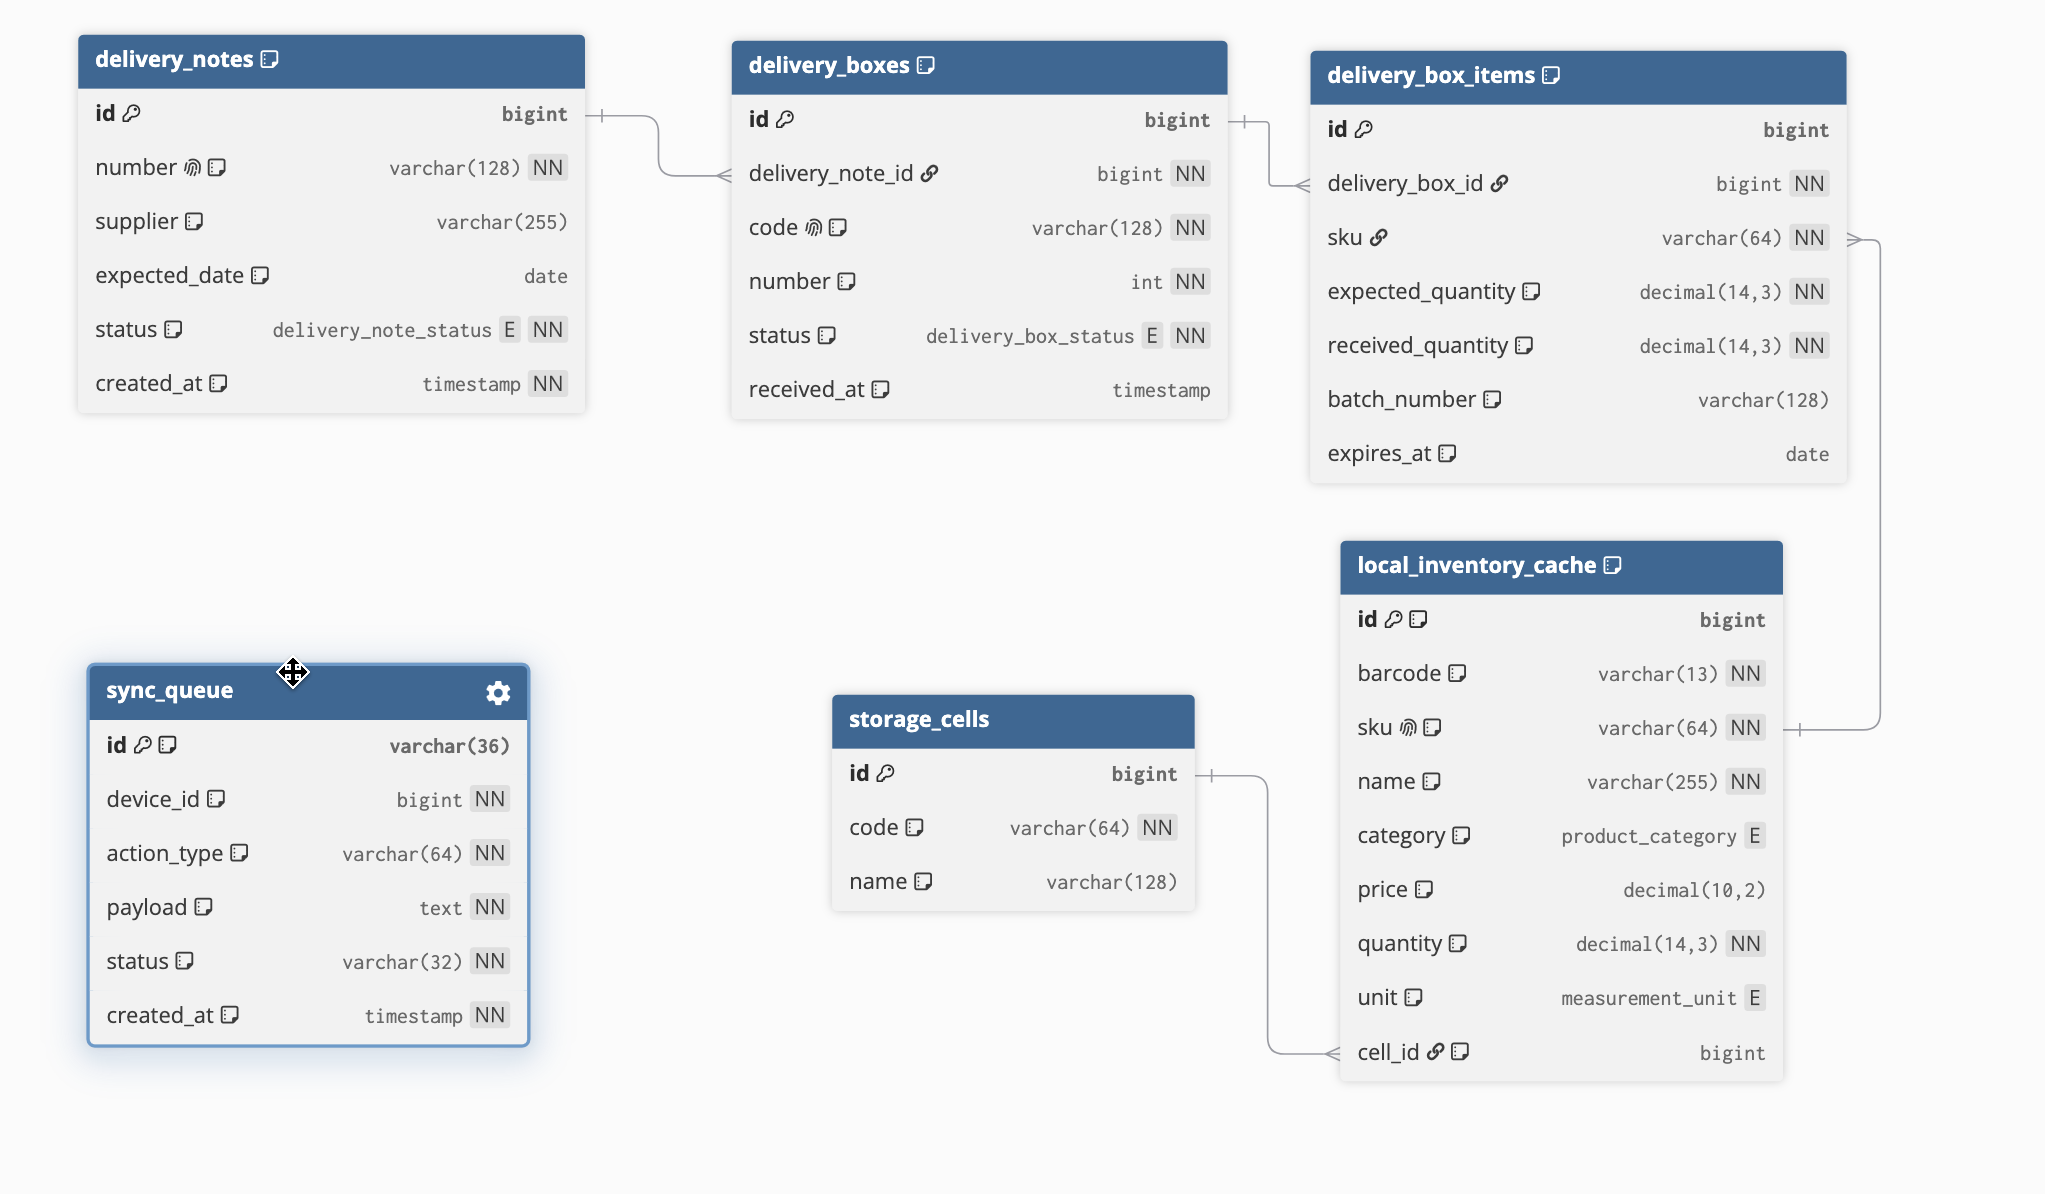
\includegraphics[width=0.90\textwidth]{assets/inventory-storage-er-diagram.png}
  \caption{Связь данных о товаре с ячейками склада}
  \label{fig:inventory-storage-er}
\end{figure}

\section{Функции приложения}

\subsection{Общие правила}

\begin{enumerate}
  \item Сотрудник видит текущую операцию, товар, ячейку и следующее действие.
  \item Сканирование само по себе не меняет данные: сотрудник подтверждает результат отдельной кнопкой.
  \item Ошибка объясняется простым текстом и не приводит к изменению остатка или результата операции.
  \item После успешного действия сотрудник видит понятный итог и может перейти к следующему заданию.
\end{enumerate}

\subsection{Рабочие сценарии}

Каждый сценарий выполняется по локально загруженному заданию. Итог подтверждается сотрудником и сохраняется на устройстве.

\begin{tabularx}{\textwidth}{L{36mm}Y}
\toprule
\textbf{Операция} & \textbf{Подробный сценарий} \\
\midrule
Приемка & Сотрудник принимает поставку от курьера: сканирует полученные коробки, сверяет их с накладной, подтверждает приемку и при необходимости фотографирует подписанную накладную в приложении. После завершения приемки коробки становятся доступны для операции размещения во внутреннем складе. Подробнее в \hyperref[scenario:receiving]{разделе~\ref{scenario:receiving} «Приемка»}. \\
Размещение & Сотрудник получает задание на размещение товаров. Для каждого товара он сканирует штрихкод товара, затем сканирует ячейку, в которую кладёт товар. После успешного сканирования ячейки товар считается размещённым на полке; сотрудник повторяет действия для следующего товара, пока не будут размещены все товары задания. Подробнее в \hyperref[scenario:placement]{разделе~\ref{scenario:placement} «Размещение»}. \\
\bottomrule
\end{tabularx}

\subsection{Условия ошибок}

\begin{tabularx}{\textwidth}{L{50mm}Y}
\toprule
\textbf{Ситуация} & \textbf{Что должен увидеть и сделать пользователь} \\
\midrule
Код не распознан & Сообщение «Не удалось считать штрихкод. Наведите камеру еще раз»; сотрудник повторяет сканирование. \\
Товар не найден & Сообщение «Товар не найден в задании»; сотрудник повторяет сканирование или возвращается к заданию без сохранения изменений. \\
Товар не подходит к заданию & Сообщение о несоответствии товару или операции; сотрудник не может подтвердить действие до сканирования корректного товара. \\
Нет доступа к камере & Объяснение необходимости доступа и кнопки «Повторить запрос» и «Открыть настройки». \\
Пользователь отменил операцию & Приложение возвращает сотрудника к заданию; локальные данные операции не изменяются. \\
Коробка уже обработана & Сообщение «Коробка уже обработана»; количество, остатки и отчёт о приёмке не меняются. \\
\bottomrule
\end{tabularx}

\subsection{Отчёт о приёмке}

После закрытия приёмки приложение сохраняет на устройстве отчёт о приёмке. В нём указываются номер задания, дата и время, список обработанных коробок, а также все отклонения. Для каждой проблемной ситуации --- например, неизвестного штрихкода, отсутствующей, лишней или повторно отсканированной коробки --- сотрудник добавляет комментарий с причиной.

Фотография подписанной накладной прикрепляется к отчёту о приёмке и сохраняется вместе с ним. После сохранения фотография доступна при просмотре отчёта.

\section{Путь пользователя}

\subsection{Карта сценариев}

Все операции используют один понятный цикл: сотрудник открывает назначенное задание, сканирует товар, проверяет данные, подтверждает результат и получает итог выполнения.

\begin{center}
\small
Выбор задания $\longrightarrow$ Накладная $\longrightarrow$ Сканирование $\longrightarrow$ Подтверждение $\longrightarrow$ Итог
\end{center}

\subsection{C01. Приемка}\label{scenario:receiving}


\begin{tabularx}{\textwidth}{L{42mm}Y}
\toprule
\textbf{Что описать} & \textbf{Сценарий приемки} \\
\midrule
Экраны & Главный экран (приемка товаров) -> Выбор накладной -> сканирование EAN-13 на коробках от поставщика -> подтверждение количества коробок -> завершение приемки фотография накладной \\
Результат & Принятые позиции фиксируются в задании; для непринятых или не соответствующих заданию товаров указывается расхождение. \\
\bottomrule
\end{tabularx}

\subsubsection{Экраны пути пользователя}

\begin{center}
\begin{tabular}{@{}ccc@{}}
\phonescreen{1}{assets/receiving/01-main.png}{Главный экран} &
\phonescreen{2}{assets/receiving/02-note-selection.png}{Выбор накладной} &
\phonescreen{3}{assets/receiving/03-receiving-task.png}{Задание на приёмку} \\
[5mm]
\phonescreen{4}{assets/receiving/04-box-confirmed.png}{Коробка принята} &
\phonescreen{5}{assets/receiving/05-box-review.png}{Проверка коробки} &
\phonescreen{6}{assets/receiving/06-discrepancy.png}{Фиксация расхождения, если было отсанировано меньше коробок чем в накладной} \\
\end{tabular}
\end{center}

\subsubsection{Экраны пути пользователя (продолжение)}

\begin{center}
\begin{tabular}{@{}ccc@{}}
\phonescreen{7}{assets/receiving/07-receiving-result.png}{Итог приёмки} &
\phonescreen{8}{assets/receiving/08-receipt-photo.png}{Фотографирование накладной} &
\phonescreen{9}{assets/receiving/09-receiving-result-with-photo.png}{Накладная прикреплена} \\
\end{tabular}
\end{center}

\subsubsection{Описание сценария}

Этап «Приёмка» предназначен для подтверждения фактически полученного товара по заранее созданному заданию на приёмку.

\begin{enumerate}
    \item На главном экране сотрудник открывает раздел «Приёмка». В списке отображаются доступные задания, ожидающие обработки.
    \item Сотрудник выбирает нужное задание на приёмку. Перед началом работы он сверяет номер задания, поставщика и сопроводительные документы с прибывшей поставкой.
    \item После открытия задания сотрудник поочерёдно сканирует штрихкоды всех коробок, входящих в поставку. Каждая коробка сканируется отдельно.
    \item После каждого сканирования приложение проверяет штрихкод и фиксирует коробку в текущем задании. На экране обновляется ход приёмки: количество отсканированных коробок, оставшиеся позиции и возможные расхождения.
    \item Если штрихкод не распознан, коробка отсутствует в задании или была отсканирована повторно, приложение сообщает об этом сотруднику. Проблемная ситуация фиксируется в отчёте о приёмке: сотрудник добавляет комментарий с причиной, а приложение не изменяет количество повторно.
    \item Сотрудник продолжает сканирование до обработки всех коробок, указанных в задании. Перед завершением он убеждается, что необработанные позиции и неподтверждённые расхождения отсутствуют.
    \item После успешного сканирования поставки сотрудник выбирает действие «Закрыть приёмку». Система сохраняет результаты, закрывает задание и фиксирует факт приёмки товара.
    \item В завершение сотрудник прикрепляет к отчёту фотографию подписанной накладной или другого подтверждающего документа. Фотография сохраняется в отчёте о приёмке и после завершения доступна при его просмотре.
\end{enumerate}

После закрытия приёмки товар считается принятым и готовым к следующей складской операции --- размещению в зоне хранения.

\subsection{C02. Размещение}\label{scenario:placement}

\subsubsection{Экраны пути пользователя}

\begin{center}
\begin{tabular}{@{}ccc@{}}
\phonescreen{1}{assets/placement/01-scan-product.jpeg}{Задание: отсканировать товар} &
\phonescreen{2}{assets/placement/02-scan-location.jpeg}{Товар распознан: отсканировать ячейку} &
\phonescreen{3}{assets/placement/03-confirm-placement.jpeg}{Ячейка совпадает: подтвердить размещение} \\
[5mm]
\phonescreen{4}{assets/placement/04-position-placed.jpeg}{Позиция размещена: сканировать следующий товар} &
\phonescreen{5}{assets/placement/05-placement-result.jpeg}{Все позиции размещены: вернуться к операциям} \\
\end{tabular}
\end{center}

\subsubsection{Описание сценария}

Этап «Размещение» предназначен для размещения товаров на полках в назначенных ячейках. К выполнению операции сотрудник приступает после завершения приёмки, когда товары становятся доступны для размещения.

\begin{enumerate}
    \item На главном экране сотрудник открывает раздел «Размещение» и выбирает нужное задание. В задании отображаются товары, которые нужно разложить по ячейкам, и ход выполнения: сколько товаров уже размещено и сколько осталось.
    \item Сотрудник берёт первый товар и сканирует его штрихкод EAN-13. Приложение находит товар в локальном каталоге и проверяет, что он входит в выбранное задание и ещё не был размещён.
    \item После успешной проверки приложение показывает ячейку, в которую нужно положить товар. Сотрудник переносит товар к этой ячейке и кладёт его на полку.
    \item Сотрудник сканирует штрихкод ячейки. Приложение сопоставляет отсканированную ячейку с ячейкой, назначенной для данного товара, и сообщает о совпадении.
    \item Сотрудник проверяет название товара и ячейку на экране, затем нажимает «Подтвердить размещение». Только после этого приложение фиксирует товар на полке и увеличивает счётчик выполненных товаров на один.
    \item Приложение показывает, что позиция размещена, и переходит к следующему неразмещённому товару. Сотрудник повторяет последовательность «сканировать товар -> сканировать ячейку -> подтвердить размещение» до тех пор, пока все товары задания не окажутся на своих местах.
    \item Если отсканирован другой товар, уже размещённый товар или неверная ячейка, приложение сообщает о несоответствии и не изменяет данные. Сотрудник проверяет маркировку и повторяет сканирование корректного товара или ячейки.
    \item Когда все товары задания размещены, приложение показывает итог операции: все товары находятся на назначенных полках, задание завершено, а сотрудник может вернуться к выбору операций.
\end{enumerate}

После завершения операции каждый товар задания считается размещённым в назначенной ячейке и доступным для дальнейших складских операций.

\begin{tabularx}{\textwidth}{L{42mm}Y}
\toprule
\textbf{Что описать} & \textbf{Сценарий размещения} \\
\midrule
Экраны & Задание: сканирование товара -> товар распознан: сканирование ячейки -> ячейка совпадает: подтверждение -> позиция размещена: следующий товар -> итог. \\
Действия сотрудника & Для каждого товара сканирует товар, сканирует назначенную ячейку, проверяет совпадение и подтверждает размещение. Повторяет действия, пока все товары задания не будут размещены. \\
Результат & После подтверждения корректной ячейки приложение фиксирует товар на этой полке, сохраняет ход выполнения на устройстве и по завершении предлагает вернуться к выбору операций. \\
\bottomrule
\end{tabularx}

\subsection{C03. Сканирование штрихкода}\label{scenario:barcode-scanning}

\begin{tabularx}{\textwidth}{L{42mm}Y}
\toprule
\textbf{Что описать} & \textbf{Сценарий сканирования штрихкода} \\
\midrule
Экраны & Экран сканирования камерой -> проверка кода -> возврат к заданию с результатом; альтернативный путь: ручной ввод EAN-13 -> проверка кода -> возврат к заданию с результатом. \\
Способы ввода & Камера является основным способом. Ручной ввод используется, если этикетка повреждена, камера недоступна или штрихкод невозможно считать. Оба способа проходят одинаковую проверку. \\
Результат & Код либо принимается для просмотра и последующего подтверждения операции, либо отклоняется с понятной причиной. Само сканирование или ручной ввод не изменяют остатки, количество и результат задания. \\
\bottomrule
\end{tabularx}

\subsubsection{Пример экранов при сканировании}


\begin{center}
\begin{tabular}{@{}cc@{}}
\phonescreen{1}{assets/scanning/01-camera-scan.png}{Сканирование камерой} &
\phonescreen{2}{assets/scanning/02-manual-entry.png}{Ручной ввод штрихкода} \\
\end{tabular}
\end{center}

\subsubsection{Описание сценария работы сканера}

Экран сканирования открывается из выбранного задания по кнопке «Сканировать». Он получает контекст текущего задания: вид операции, ожидаемый товар, требуемое количество, исходную и целевую ячейки при их наличии.

\begin{enumerate}
    \item При открытии основного экрана запускается камера устройства. Сотрудник видит изображение с камеры, рамку для штрихкода. На экране доступны действия «Отмена» и переход к ручному вводу данных штрих кода.
    \item Сотрудник размещает этикетку коробки в рамке. После распознавания камера приостанавливается, чтобы один и тот же штрихкод не был считан несколько раз подряд. Приложение подаёт короткий звуковой или вибрационный сигнал и начинает проверку кода.
    \item Считанное значение очищается от пробелов по краям и проверяется как EAN-13: оно должно состоять из 13 цифр и иметь корректную контрольную цифру. Коды других форматов, неполные коды и коды с ошибочной контрольной цифрой не принимаются.
    \item Для корректного EAN-13 приложение ищет конкретный товар в локальном каталоге устройства, затем проверяет, соответствует ли товар текущему заданию и доступен ли он для выбранной операции. До завершения этой проверки сотруднику не показывается подтверждение операции.
    \item Если камера не может считать этикетку, сотрудник выбирает ручной ввод. На отдельном экране он вводит 13 цифр EAN-13 и нажимает «Проверить». Ручной код проходит ровно те же проверки, что и считанный камерой; ручной ввод не является способом обойти проверку товара или задания.
    \item Сотрудник может отменить сканирование или ручной ввод в любой момент. Приложение возвращает его в задание без сохранения кода и без изменения данных.
\end{enumerate}

\clearpage
\begin{landscape}
\subsubsection{Блок-схема обработки результата сканирования}

Проверки выполняются до показа карточки товара и до подтверждения операции.

\begin{center}
  \vspace*{\fill}
  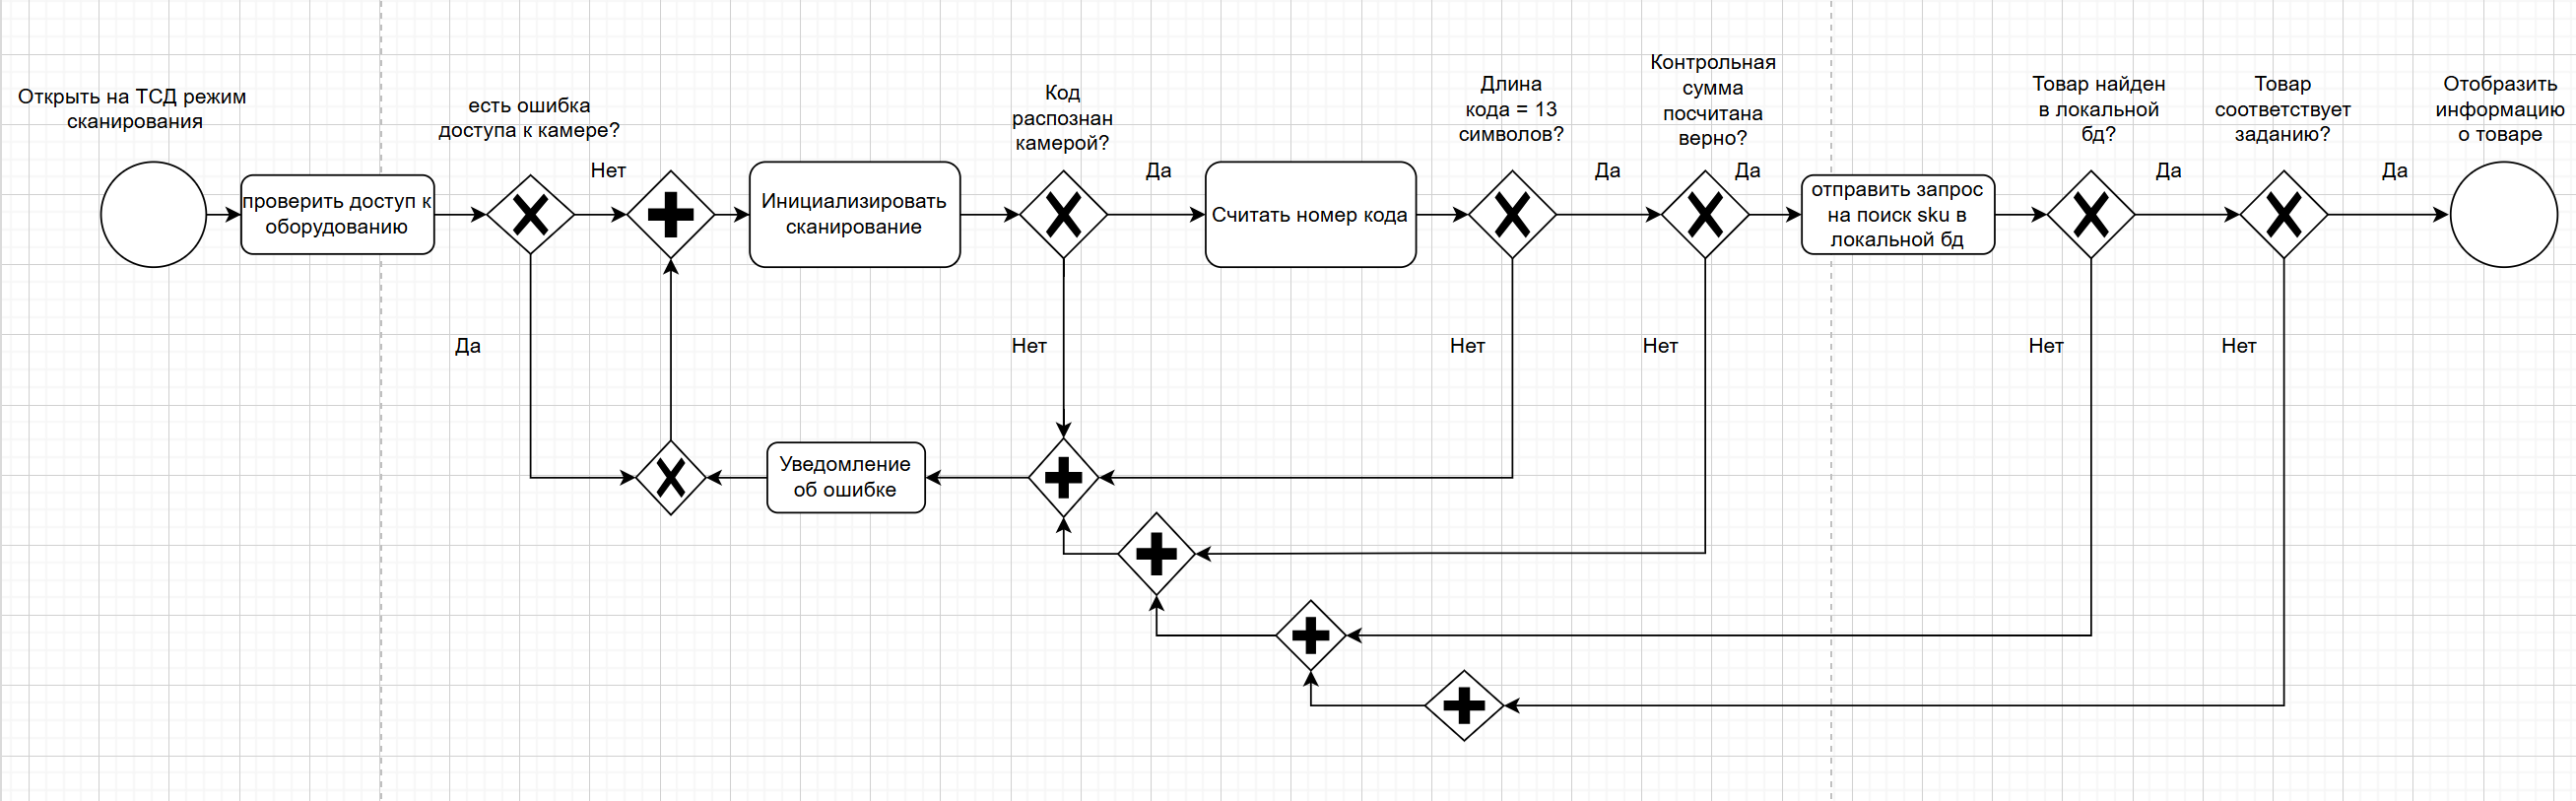
\includegraphics[width=\linewidth,keepaspectratio]{assets/scanning/scanning-result-processing-flow.png}
  \par\smallskip
  \refstepcounter{figure}\small\textbf{\figurename~\thefigure~---} Процесс сканирования и обработки результата
  \label{fig:scanning-result-processing}
  \vspace*{\fill}
\end{center}
\end{landscape}
\clearpage

\subsubsection{Обработка сложных ситуаций}

\begin{longtable}{L{44mm}L{112mm}}
\toprule
\textbf{Ситуация} & \textbf{Поведение приложения и действие сотрудника} \\
\midrule
\endfirsthead
\toprule
\textbf{Ситуация} & \textbf{Поведение приложения и действие сотрудника} \\
\midrule
\endhead
Штрихкод не распознан камерой & На экране выводится сообщение «Не удалось считать штрихкод. Наведите камеру ещё раз». Данные не изменяются, камера остаётся доступной для повторной попытки; сотрудник может переключиться на ручной ввод. \\
Распознан неподдерживаемый формат & Приложение сообщает «Нужен штрихкод EAN-13». Код не передаётся в задание, камера возобновляет работу после сообщения. \\
Некорректный EAN-13 & При ручном вводе поле принимает только цифры; при нажатии «Проверить» приложение сообщает о необходимости ввести 13 цифр с верной контрольной цифрой. При сканировании камера возобновляет работу. \\
Товар не найден в каталоге & Отображается сообщение «Товар не найден в локальном каталоге». Код не принимается, количество и остатки не меняются. Сотрудник проверяет этикетку, повторяет сканирование или передаёт ситуацию ответственному сотруднику. \\
Товар не соответствует заданию & Приложение сообщает, что отсканирован неподходящий товар, и показывает ожидаемый товар. Подтверждение операции недоступно до сканирования корректной коробки. \\
Коробка отсканирована повторно & Если коробка уже была принята или размещена в рамках текущего задания, приложение выводит сообщение «Коробка уже обработана». Повторное сканирование не увеличивает количество, не меняет остатки и не создаёт вторую запись операции; сотрудник сканирует следующую коробку. \\
Задание уже завершено & Приложение сообщает «Задание уже выполнено» и не принимает код. Сотрудник возвращается к списку заданий и выбирает актуальное задание. \\
Недостаточно товара для операции & Приложение сообщает, что товара в исходной ячейке недостаточно, и не позволяет подтвердить действие. Сотрудник проверяет предыдущее размещение или обращается к ответственному сотруднику. \\
Нет разрешения на камеру & Экран объясняет, что для сканирования нужен доступ к камере, и предлагает кнопки «Повторить» и «Открыть настройки Android». До выдачи разрешения доступен ручной ввод и отмена. \\
Камера занята или недоступна & Отображается понятное сообщение с рекомендацией закрыть другое приложение, использующее камеру. Сотрудник может повторить запуск камеры, перейти к ручному вводу или отменить действие. \\
\bottomrule
\end{longtable}

\section{Локальные данные и сканер}

\subsection{Хранение и загрузка данных}

\begin{tabularx}{\textwidth}{L{48mm}Y}
\toprule
\textbf{Вопрос} & \textbf{Решение} \\
\midrule
Где хранятся данные? & Каталог товаров, ячейки, задания, результаты операций и отчёты о приёмке хранятся только в локальной базе данных устройства. \\
Как данные попадают в приложение? & Перед началом работы в приложение импортируются подготовленные файлы со справочником товаров, ячейками и заданиями. Внешняя учётная система не подключается. \\
Что содержит штрихкод? & Используется EAN-13. По отсканированному коду приложение находит конкретный товар в локальном каталоге и проверяет его соответствие открытому заданию. \\
Когда данные меняются? & Только после явного подтверждения сотрудником. Сканирование и ручной ввод только проверяют код. \\
Где хранится фото накладной? & Фотография подписанной накладной сохраняется в отчёте о приёмке и доступна при его просмотре. \\
\bottomrule
\end{tabularx}

\subsection{Поведение сканера}

\begin{tabularx}{\textwidth}{L{48mm}Y}
\toprule
\textbf{Ситуация} & \textbf{Решение} \\
\midrule
Основной способ сканирования & Камера Android-устройства; распознавание EAN-13 выполняется без сети. \\
Альтернативный способ & Сотрудник может вручную ввести 13 цифр EAN-13. Ручной ввод проходит такую же проверку, как код с камеры. \\
Успешное считывание & Камера приостанавливается, код проверяется в локальном каталоге и в контексте открытого задания. Затем сотрудник возвращается к подтверждению операции. \\
Ошибка считывания & Приложение показывает понятную причину ошибки, не изменяет локальные данные и позволяет повторить сканирование или перейти к ручному вводу. \\
Замена сканера & Бизнес-операции используют единый интерфейс сканера; камерная и аппаратная реализации не меняют сценарии экранов. \\
\bottomrule
\end{tabularx}

\section{Критерии приёмки}

Продукт считается готовым к демонстрации, если все экраны и действия выполняются в соответствии с описанием в настоящем ТЗ.

\begin{tabularx}{\textwidth}{L{48mm}Y}
\toprule
\textbf{Проверяемая часть} & \textbf{Критерий готовности} \\
\midrule
Приёмка & Сотрудник проходит путь C01: открывает локальное задание, сканирует коробки, фиксирует отклонения в комментариях отчёта, закрывает приёмку и прикрепляет фотографию подписанной накладной. \\
Размещение & Сотрудник проходит путь C02: выбирает задание, сканирует коробку и ячейку, подтверждает размещение и видит сохранённый на устройстве результат. \\
Сканирование & Сотрудник проходит путь C03 камерой и вручную. Приложение принимает только корректный EAN-13, находит товар в локальном каталоге, не принимает неподходящий или повторный код и не меняет данные до подтверждения. \\
Локальные данные & После импорта файлов приложение открывает задания и справочник без подключения к внешней учётной системе; результат подтверждённой операции доступен на устройстве. \\
Фотография накладной & После сохранения фотография доступна при просмотре отчёта о приёмке. \\
\bottomrule
\end{tabularx}


\end{document}
